\begin{center}

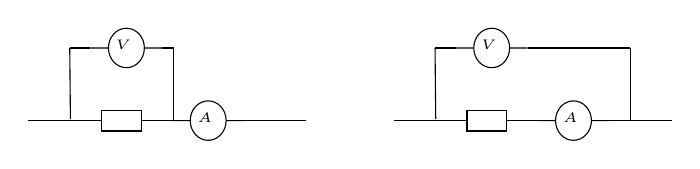
\begin{tikzpicture}[x=0.75pt,y=0.75pt,yscale=-1,xscale=1]
%uncomment if require: \path (0,300); %set diagram left start at 0, and has height of 300

%Shape: Output [id:dp5029694724185756] 
\draw   (238.05,164.5) .. controls (238.05,159.25) and (241.92,155) .. (246.7,155) .. controls (251.48,155) and (255.35,159.25) .. (255.35,164.5) .. controls (255.35,169.75) and (251.48,174) .. (246.7,174) .. controls (241.92,174) and (238.05,169.75) .. (238.05,164.5) -- cycle (229.4,164.5) -- (238.05,164.5) (264,164.5) -- (255.35,164.5) ;
%Straight Lines [id:da5974052849252933] 
\draw    (224.6,129.5) -- (230,129.5) ;
%Shape: Output [id:dp8316238314489566] 
\draw   (198.65,129.5) .. controls (198.65,124.25) and (202.52,120) .. (207.3,120) .. controls (212.08,120) and (215.95,124.25) .. (215.95,129.5) .. controls (215.95,134.75) and (212.08,139) .. (207.3,139) .. controls (202.52,139) and (198.65,134.75) .. (198.65,129.5) -- cycle (190,129.5) -- (198.65,129.5) (224.6,129.5) -- (215.95,129.5) ;
%Straight Lines [id:da8770858852700789] 
\draw    (180,129.5) -- (190,129.5) ;
%Shape: Resistor [id:dp38586331306767896] 
\draw   (195.4,159.5) -- (214.6,159.5) -- (214.6,169.5) -- (195.4,169.5) -- (195.4,159.5) -- cycle (190,164.5) -- (195.4,164.5) (214.6,164.5) -- (220,164.5) ;
%Straight Lines [id:da6656965163696436] 
\draw    (190,164.5) -- (160,164.5) ;
%Straight Lines [id:da878906269405904] 
\draw    (230,164.5) -- (220,164.5) ;
%Straight Lines [id:da9520335954325532] 
\draw    (230,129.5) -- (230,164.5) ;
%Straight Lines [id:da14449988398828695] 
\draw    (294,164.5) -- (264,164.5) ;
%Straight Lines [id:da6761861997187404] 
\draw    (180,129.5) -- (180.33,163.85) ;
%Shape: Output [id:dp49152989281976267] 
\draw   (414.05,164.5) .. controls (414.05,159.25) and (417.92,155) .. (422.7,155) .. controls (427.48,155) and (431.35,159.25) .. (431.35,164.5) .. controls (431.35,169.75) and (427.48,174) .. (422.7,174) .. controls (417.92,174) and (414.05,169.75) .. (414.05,164.5) -- cycle (405.4,164.5) -- (414.05,164.5) (440,164.5) -- (431.35,164.5) ;
%Straight Lines [id:da025922891978220397] 
\draw    (400.6,129.5) -- (450,129.5) ;
%Shape: Output [id:dp10986368699785243] 
\draw   (374.65,129.5) .. controls (374.65,124.25) and (378.52,120) .. (383.3,120) .. controls (388.08,120) and (391.95,124.25) .. (391.95,129.5) .. controls (391.95,134.75) and (388.08,139) .. (383.3,139) .. controls (378.52,139) and (374.65,134.75) .. (374.65,129.5) -- cycle (366,129.5) -- (374.65,129.5) (400.6,129.5) -- (391.95,129.5) ;
%Straight Lines [id:da6881881555017568] 
\draw    (356,129.5) -- (366,129.5) ;
%Shape: Resistor [id:dp538700598242954] 
\draw   (371.4,159.5) -- (390.6,159.5) -- (390.6,169.5) -- (371.4,169.5) -- (371.4,159.5) -- cycle (366,164.5) -- (371.4,164.5) (390.6,164.5) -- (396,164.5) ;
%Straight Lines [id:da9465905183870709] 
\draw    (366,164.5) -- (336,164.5) ;
%Straight Lines [id:da06582730048417962] 
\draw    (406,164.5) -- (396,164.5) ;
%Straight Lines [id:da4945798647049118] 
\draw    (450,129.5) -- (450,164.5) ;
%Straight Lines [id:da23103050393206437] 
\draw    (470,164.5) -- (440,164.5) ;
%Straight Lines [id:da28372038020800505] 
\draw    (356,129.5) -- (356.33,163.85) ;

% Text Node
\draw (240.4,159.5) node [anchor=north west][inner sep=0.75pt]  [font=\tiny] [align=left] {$\displaystyle A$};
% Text Node
\draw (201,124.5) node [anchor=north west][inner sep=0.75pt]  [font=\tiny] [align=left] {$\displaystyle V$};
% Text Node
\draw (416.4,159.5) node [anchor=north west][inner sep=0.75pt]  [font=\tiny] [align=left] {$\displaystyle A$};
% Text Node
\draw (377,124.5) node [anchor=north west][inner sep=0.75pt]  [font=\tiny] [align=left] {$\displaystyle V$};


\end{tikzpicture}

\end{center}